%% abtex2-modelo-trabalho-academico.tex, v-1.9.7 laurocesar
%% Copyright 2012-2018 by abnTeX2 group at http://www.abntex.net.br/ 
%%
%% This work may be distributed and/or modified under the
%% conditions of the LaTeX Project Public License, either version 1.3
%% of this license or (at your option) any later version.
%% The latest version of this license is in
%%   http://www.latex-project.org/lppl.txt
%% and version 1.3 or later is part of all distributions of LaTeX
%% version 2005/12/01 or later.
%%
%% This work has the LPPL maintenance status `maintained'.
%% 
%% The Current Maintainer of this work is the abnTeX2 team, led
%% by Lauro César Araujo. Further information are available on 
%% http://www.abntex.net.br/
%%
%% This work consists of the files abntex2-modelo-trabalho-academico.tex,
%% abntex2-modelo-include-comandos and abntex2-modelo-references.bib
%%

% ------------------------------------------------------------------------
% ------------------------------------------------------------------------
% abnTeX2: Modelo de Trabalho Academico (tese de doutorado, dissertacao de
% mestrado e trabalhos monograficos em geral) em conformidade com 
% ABNT NBR 14724:2011: Informacao e documentacao - Trabalhos academicos -
% Apresentacao
% ------------------------------------------------------------------------
% ------------------------------------------------------------------------

\documentclass[
	% -- opções da classe memoir --
	12pt,				% tamanho da fonte
	openright,			% capítulos começam em pág ímpar (insere página vazia caso preciso)
	oneside,			% para impressão em recto e verso. Oposto a oneside
	a4paper,			% tamanho do papel. 
	% -- opções da classe abntex2 --
	%chapter=TITLE,		% títulos de capítulos convertidos em letras maiúsculas
	%section=TITLE,		% títulos de seções convertidos em letras maiúsculas
	%subsection=TITLE,	% títulos de subseções convertidos em letras maiúsculas
	%subsubsection=TITLE,% títulos de subsubseções convertidos em letras maiúsculas
	% -- opções do pacote babel --
	english,			% idioma adicional para hifenização
	french,				% idioma adicional para hifenização
	spanish,			% idioma adicional para hifenização
	brazil				% o último idioma é o principal do documento
	]{elementos/customizacao}

% ---
% Compila o Índice
% ---
\makeindex
% ---

% ----
% Início do documento
% ----
\begin{document}

% Seleciona o idioma do documento (conforme pacotes do babel)
%\selectlanguage{english}
\selectlanguage{brazil}

% Retira espaço extra obsoleto entre as frases.
\frenchspacing 

% ----------------------------------------------------------
% ELEMENTOS PRÉ-TEXTUAIS
% ----------------------------------------------------------
% \pretextual

% ---
% Capa
% ---
% --- 
% Alterando a capa
% --- 
\begin{capa}% \center
	\begin{center}
		\ABNTEXchapterfont\muctbf{\imprimirinstituicao} \\ \muctbf{Pró-Reitoria Acadêmica – PROAC} \\ \muctbf{\nomecurso}


			\vspace*{5cm}

			{\ABNTEXchapterfont\muctbf\imprimirautor}

			\vfill
				\ABNTEXchapterfont\bfseries\muctbf\imprimirtitulo
			\vfill

			\muctbf \imprimirlocal

			\muctbf \imprimirdata
	\end{center}
\end{capa}
% --- 



% --- 
% Folha de Rosto
% --- 
\makeatletter

\renewcommand{\folhaderostocontent}{
	\begin{center}
		{\ABNTEXchapterfont\muctbf\imprimirtitulo}

		\vspace*{2cm}

		\abntex@ifnotempty{\imprimirpreambulo}{%
			\hspace{.45\textwidth}
		\begin{minipage}{.5\textwidth}
			\SingleSpacing
			\imprimirpreambulo
		\end{minipage}%
		\vspace*{\fill}
		}%

		\vspace*{\fill}

		\muctbf{\imprimirlocal}

		\muctbf{\imprimirdata}
	\end{center}
}

\makeatother

% ---

% ---
% Folha de rosto
% (o * indica que haverá a ficha bibliográfica)
% ---
\imprimirfolhaderosto
% ---

% ---
% Inserir errata
% ---
%\input{pretextuais/errata}
%\imprimirerrata
% ---

% ---
% Inserir a ficha bibliográfica
% ---
\input{pretextuais/fichacatalografica}
% ---

% ---
% Inserir folha de aprovação
% ---
\input{pretextuais/folhaaprovacao}
% ---

% ---
% Dedicatória
% ---
\begin{dedicatoria}
	\vspace*{\fill}
		\centering
		\noindent
		\textit{ 
			Dedico este trabalho ao meu professor orientador MSc. \imprimirorientador\ por me acolher e aconselhar passando seus conhecimentos sem pestanejos e me aceitando como último orientando antes de sua jornada em busca do título de doutorado. Dedico também ao professor MSc. Hugo Vieira Lucena de Souza por todos seus conselhos, ensinamentos e correções que foram possível para conclusão deste título. Também dedico este trabalho e ao professor Erick France Meira de Souza por sua amizade, suporte e preciosos conselhos dados.
		} \vspace*{\fill}
\end{dedicatoria}

% ---

% ---
% Agradecimentos
% ---
\begin{agradecimentos}
	Gostaria de agradecer minha avó Carminha (in memorian) e primo Luiz Felipe Abreu (in memorian).

			Gostaria de agradecer aos meu pais Mathura Pati Devi Das e Subala Das por sempre prezar e batalhar pela educação dos seu filhos, sem medir esforços para que todos pudesse se graduar e obter a formação acadêmica necessária.

			Meus agradecimentos também a minhas irmã Jahnavi Caran por me apoiar, dar suporte e aconselhar na minha trajetória acadêmica. Meus sinceros agradecimentos e minha eterna gratidão, irmã.


			A todos os professores e pessoas não citadas diretamente neste texto, mas que participaram e contribuíram de alguma forma com a minha formação, meu muito obrigado.

	\emph{\abnTeX}\footnote{\url{http://groups.google.com/group/abntex2}}
	\emph{latex-br}\footnote{\url{http://groups.google.com/group/latex-br}} 
	\footnote{\url{http://www.cpai.unb.br/}}

\end{agradecimentos}

% ---

% ---
% Epígrafe
% ---
\begin{epigrafe}
	\vspace*{\fill}
	\begin{flushright}
		\textit{``este trabalho é dedicado a uma criança a qual sempre falou que seria um cientista. Ele ainda vive.}
	\end{flushright}
\end{epigrafe}

% ---

% ---
% RESUMOS
% ---
% resumo em português
\setlength{\absparsep}{18pt} % ajusta o espaçamento dos parágrafos do resumo
\begin{resumo}
	Políticas públicas de transparência e fiscalização são essenciais para que o cidadão disponha de controle na fiscalização de gastos públicos. Porém, tais cidadães certamente podem utilizar a \textit{internet} como canal mediador entre as entidade portadora dos dados para fiscalização pública e o cidadão que atua como fiscal neste cenário. A \textit{internet} acaba excluindo, assim, pessoas leigas em elementos com teor tecnológico.

Em vista disso, este trabalho propõe a criação de uma aplicação que auxilie na busca dos dados dados públicos persistidos em uma base de dados. Para facilitar a utilização, será utilizada a linguagem natural possibilitando a pessoas leigas em assuntos de conhecimentos tecnológicos, possam utilizar a aplicação e poder ajudar na fiscalização dos gastos governamentais.

Para o processamento da linguagem natural, será utilizado a suite de \textit{software} Language Understanding Intelligent Service (LUIS) é uma suite de software pertencente a um dos Serviços Cognitivos da Microsoft que utiliza um ramo da Inteligência Artificial (IA) chamado Processamento de Linguagem Natural (PLN) (MAYO, 2017). Essa suite, possibilita que aplicações possam adquirir certo grau de inteligência. Formando assim, seu objetivo central

	\textbf{Palavras-chave}: latex. abntex. editoração de texto.

\end{resumo}

\begin{enumerate}
\item Tecnologia no problema
\item Apresentar limitação das aplicações existentes
\item Mostrar que não há aplicações direcionadas a este propósito
\item Mostrar aplicação (solução) que ajudará no problema apresentado
\item Falar sobre a metodologia
\item Falar sobre a o desenvolvimento da aplicação seguindo a metodologia
\end{enumerate}


\newpage
{\fontsize{17}{0}\selectfont Construção do Resumo}
\begin{itemize}
\item Indicativo sobre o trabalho e não sobre o conteúdo do trabalho
\item Entre 150 e 500 palavras
\item Não usar abreviações, símbolos, formulas, equações ou diagramas a não ser que seje estritamente indispensáveis
\item Não usar citações
\item Não faça mais de um paragrafo
\item Não crie tópicos
\item Sem frases negativas
\item Após o título do trabalho e nome dos autores
\item Primeira frase indica o tema do trabalho
\item Informar os objetivos geral e específicos, metodologia, resultados 
\item 3 a 5 palavras chaves que represente a essência do trabalho separadas por pontos
\end{itemize}

{\fontsize{17}{0}\selectfont Partes do Resumo}
\begin{itemize}
\item Introdução

Objetivos e relevância do trabalho do trabalho. 
\item Metodologia

Elementos essenciais do método de pesquisa
\item Resultados

Principais resultados ou de maior destaque que pode ser representativo da pesquisa
\item Discussão
\item Conclusão

Contribuição e limites do trabalho
\end{itemize}

{\fontsize{17}{0}\selectfont Normas ABNT resumo}
\begin{itemize}
\item Frases afirmativas, curtas, escritas em voz ativa e na terceira pessoa do singular
\item Texto claro, conciso, seguir uma ordem lógica e sem completamente fiel ao trabalho
\item Deve mencionar o tema, objetivo, métodos, resultados e conclusões
\item Deve indicar, no fim, palavras chaves
\end{itemize}

\include{pretextuais/resumos/resumoig}
% ---

% ---
% inserir lista de ilustrações
% ---
\pdfbookmark[0]{\listfigurename}{lof}
\listoffigures*
\cleardoublepage
% ---

% ---
% inserir lista de quadros
% ---
%\pdfbookmark[0]{\listofquadrosname}{loq}
%\listofquadros*
%\cleardoublepage
% ---

% ---
% inserir lista de tabelas
% ---
%\pdfbookmark[0]{\listtablename}{lot}
%\listoftables*
%\cleardoublepage
% ---

% ---
% inserir lista de abreviaturas e siglas
% ---
\begin{siglas}
\item[API] Application Programming Interface
\item[LUIS] Language Understanding Intelligent Service
\item[JSON] JavaScript Object Notation
\item[IA] Inteligência Artificial
\item[PLN] Processamento de Linguagem Natural 
\end{siglas}

% ---

% ---
% inserir lista de símbolos
% ---
%\input{pretextuais/simbolos}
% ---

% ---
% inserir o sumario
% ---
\pdfbookmark[0]{\contentsname}{toc}
\tableofcontents*
\cleardoublepage
% ---



% ----------------------------------------------------------
% ELEMENTOS TEXTUAIS
% ----------------------------------------------------------
\textual

% ----------------------------------------------------------
% Introdução (exemplo de capítulo sem numeração, mas presente no Sumário)
% ----------------------------------------------------------
\chapter{Introdução}
A barreira do aprendizado para a interação entre homem e sistemas computacionais até os dias atuais ainda é um obstáculo a ser conquistado devido a necessidade de tempo e interesse por parte dos usuário. \cite{Barbosa:2010} afirmam que usuários que se dispõem a aprender novos sistemas interativos com características únicas e distintas precisam dispor de tempo e interesse para posteriormente ser capazes de usufruir e usar as funcionalidades deste sistema.

Consequentemente, pessoas que não possuem hábito de utilização da internet e sem muito conhecimento técnico em manusear softwares de acesso podem deixar de participar de eventos, oportunidades e movimentos que utilizam como meio à internet. Pessoas com estas características podem se ausentar da participação no controle sobre a Administração Pública atuando na verificação, acompanhamento e fiscalização da regularidade de gastos públicos devido a se depararem com barreiras até mesmo no momento do recolhimento dos dados públicos que utilizam como canal mediador a internet.

No que se refere a fiscalização, com a promulgação da Constituição de 1988, o Brasil se classificou se como um Estado Democŕatico de Direito onde uma de suas características, para este tipo de estado, é a participação popular no controle sobre a Administração Pública. Neste sentido, o cidadão tem o poder de acompanhar e fiscalizar a regularidade dos atos governamentais juntamente com os órgãos institucionais legalmente criados para esta finalidade \cite{Arruda:2010}.

Tendo em vista que em 2000 foi promulgada a Lei de Responsabilidade Fiscal, que entre muito outros pontos, no artigo 48, definiu que as prestações de contas e outros instrumentos de transparência da gestão fiscal pública devem ter ampla divulgação, inclusive em meios eletrônicos de acesso público. Porém, todo benefício gerado a partir das regras impostas por esta lei, podem não ser devidamente aproveitadas por cidadãos que não possuem conhecimento prévio na utilização da internet.

Surgindo assim a pergunta central que este trabalho se propõe a intervir: como facilitar o acesso às informações públicas com o propósito que pessoas, sem conhecimento técnico em sistemas computacionais, possam auxiliar no processo de fiscalização de gastos governamentais, ajudando assim a diminuir os índices de corrupção no país?

\section{Justificativa}
A partir da promulgação da Lei de Acesso à Informação, Lei nº 12.527/2011, foi garantido o direito constitucional de acesso às informações públicas, possibilitando que qualquer pessoa física ou jurídica, sem a necessidade de apresentar motivos, receba informações públicas de órgãos e entidades. Desta forma, surgem novos mecanismos os quais possibilitam a participação do cidadão na fiscalização de gastos públicos e combate à corrupção.

		A melhoria do acesso à informação pública e a criação de regras que permitem a disseminação de informações produzidas pelo governo reduzem os abusos que podem ser cometidos \cite{Islam:2002}. Porém, tais dados estão mais disponíveis em sistemas computacionais mediante a internet, utilizando-se muitas vezes de ferramentas carentes de parametrização ou disponibilização dos dados em grandes planilhas, dificultando assim o entendimento por parte de não-especialistas em informática.

		Na tentativa de melhorar a divulgação dos dados públicos, o Ministério da Transparência em conjunto com a Controladoria-Geral da União, em 2004, criou o site Portal da Transparência do Governo Federal que possibilita o acesso livre, no qual o cidadão pode encontrar informações sobre como o dinheiro público é utilizado, além de se informar sobre assuntos relacionados à gestão pública do Brasil.  Ainda assim, o problema de acesso por pessoas sem muitos conhecimentos técnicos sobre internet e como utilizá-la continua a existir.

		Como forma de intervenção, este trabalho sugere a utilização de linguagem natural para busca e manipulação dos dados em bases de dados disponibilizadas pelo Governo Federal. “O processamento de linguagem natural permite ao computador compreender e reagir a declarações e comandos de voz realizados em uma linguagem natural” \cite[p. 508]{Stair:2015}. Para tal, este trabalho propõe a utilização do serviço de API de reconhecimento vocal Language Understanding Intelligent Service (LUIS) que aplica inteligência de aprendizado personalizado de máquina a um texto de linguagem natural e extrai informações relevantes a futuras aplicações.  Para isso, este trabalho também propõe a utilização da ferramenta Elasticsearch que, entre muitas funcionalidades, possui recursos e tecnologias que permitem realizar consultas através de índices em grandes volumes de dados em tempo real \cite{Gil:2010}.


\section{Objetivos}
\subsection{Objetivo Geral}
Desenvolver uma ferramenta que utiliza processamento de linguagem natural, interface gráfica e busca em índices a fim de facilitar o acesso aos dados governamentais públicos disponíveis.

\subsection{Objetivos Específicos}
Realizar um estudo acerca do conjuntos tecnologias utilizadas para a criação de um sistema de interação descrevendo suas características e possibilidades possíveis de utilização para se atingir o objetivo geral.

Replicar uma base de dados públicos governamentais a fim de indexar as informações localmente;

Gerar o treinamento do algoritmo do LUIS, produto da Microsoft, a fim de entender e diferenciar ações diversas a serem realizadas.

Gerar versão de teste, utilizando o texto de entrada no algoritmo do LUIS, e gerando consultas parametrizadas e customizadas para retornar índices da base de dados replicada.


\section{Metodologia}
“Método é o conjunto das atividades sistemáticas e racionais que, com maior segurança e economia, permite alcançar o objetivo de produzir conhecimentos válidos e verdadeiros, traçando o caminho a ser seguido, detectando erros e auxiliando as decisões” \cite[p. 79]{Lakatos:2010}. As autoras descrevem também que a ciência caracteriza-se pela utilização de métodos científicos e que estes não são de uso exclusivo pela ciência. Porém, não é possível a ciência estar apartado do emprego de métodos científicos \cite{Lakatos:2010}.

Com o objetivo de facilitar análise e avaliações futuras, este trabalho é dividido sobre a características dos tipos de pesquisas que foram aplicada do processo de construção deste trabalho.

Este trabalho se classifica como pesquisa exploratória pois entre outros fatores é tentado proporcionar maior familiaridade com as ferramentas utilizadas pela solução de software proposta. Realizando para isso,  levantamento bibliográficos com o propósito de explicar e expor possibilidades proporcionadas por estas ferramentas. Como \cite{Gil:2010} explana que o levantamento bibliográfico utilizada pelas pesquisas exploratórias é uma das maneiras utilizadas para  a coleta de dados relevantes.

Este trabalho também se classifica como uma pesquisa aplicada devido ao propósito ser uma possível abordagem ao problema identificado da dificuldade de acesso às informações públicas em que pessoas, sem conhecimento técnico em sistemas computacionais, possam posteriormente auxiliar no processo de fiscalização de gastos governamentais. \cite[p. 25]{Gil:2010} “pesquisa aplicada, abrange estudos elaborados com a finalidade de resolver problemas identificados no âmbito das sociedades em que os pesquisadores vivem”.

Com o intuito a avaliações futuras sobre a qualidade dos resultados  mostrados neste trabalho, foi adotado a análise e interpretação dos dados expostos de forma qualitativa. Devido a descrição dos resultados serem em formas verbais e não em termos numéricos como proposto pelas pesquisas quantitativa. \cite[p. 39]{Gil:2010} “Nas pesquisas quantitativas os resultados são apresentadas em termos numéricos e, nas qualitativas, mediante descrições verbais”.

Os procedimentos adotados na análise, interpretação e coleta dos dados exposto neste trabalho são realizados de forma bibliográfica e experimental. A forma bibliográfica se dá pela referenciação de dados através de citações de materiais já publicados. Enquanto que a experimental se dá pela adoção de testes de caso de uso utilizado para demonstrar a eficácia do software proposto para intervenção ao problema.


\section{Organização do Trabalho}
Após esse capítulo introdutório, o conteúdo deste trabalho organiza-se da seguinte forma:
	\begin{itemize}
		\item{Capítulo 2 - \uppercase{Conjuntos de tecnologias utilizadas}: apresentará o conjunto de ferramentas que vão possibilitar a criação da ferramenta proposta.}
		\item{Capítulo 3 - \uppercase{Arquitetura da solução}: apresentará a arquitetura da solução proposta, detalhando seu fluxo de funcionamento e diagrama para melhor compreensão da aplicação.}
		\item{Capítulo 4 - \uppercase{Replica base de dados públicos governamentais}: apresentará a arquitetura da solução proposta, detalhando seu fluxo de funcionamento e diagrama para melhor compreensão da aplicação.}
	\end{itemize}


%Este documento e seu código-fonte são exemplos de referência de uso da classe
%\textsf{abntex2} e do pacote \textsf{abntex2cite}. O documento 
%exemplifica a elaboração de trabalho acadêmico (tese, dissertação e outros do
%gênero) produzido conforme a ABNT NBR 14724:2011 \emph{Informação e documentação
%- Trabalhos acadêmicos - Apresentação}.
%
%A expressão ``Modelo Canônico'' é utilizada para indicar que \abnTeX\ não é
%modelo específico de nenhuma universidade ou instituição, mas que implementa tão
%somente os requisitos das normas da ABNT. Uma lista completa das normas
%observadas pelo \abnTeX\ é apresentada em \citeonline{abntex2classe}.
%
%Sinta-se convidado a participar do projeto \abnTeX! Acesse o site do projeto em
%\url{http://www.abntex.net.br/}. Também fique livre para conhecer,
%estudar, alterar e redistribuir o trabalho do \abnTeX, desde que os arquivos
%modificados tenham seus nomes alterados e que os créditos sejam dados aos
%autores originais, nos termos da ``The \LaTeX\ Project Public
%License''\footnote{\url{http://www.latex-project.org/lppl.txt}}.
%
%Encorajamos que sejam realizadas customizações específicas deste exemplo para
%universidades e outras instituições --- como capas, folha de aprovação, etc.
%Porém, recomendamos que ao invés de se alterar diretamente os arquivos do
%\abnTeX, distribua-se arquivos com as respectivas customizações.
%Isso permite que futuras versões do \abnTeX~não se tornem automaticamente
%incompatíveis com as customizações promovidas. Consulte
%\citeonline{abntex2-wiki-como-customizar} para mais informações.
%
%Este documento deve ser utilizado como complemento dos manuais do \abnTeX\ 
%\cite{abntex2classe,abntex2cite,abntex2cite-alf} e da classe \textsf{memoir}
%\cite{memoir}. 
%
%Esperamos, sinceramente, que o \abnTeX\ aprimore a qualidade do trabalho que
%você produzirá, de modo que o principal esforço seja concentrado no principal:
%na contribuição científica.
%
%Equipe \abnTeX 
%
%Lauro César Araujo


% ----------------------------------------------------------
% PARTE
% ----------------------------------------------------------
\part{Preparação da pesquisa}
% ----------------------------------------------------------
% Capitulo com exemplos de comandos inseridos de arquivo externo 

%\include{abntex2-modelo-include-comandos}
% ----------------------------------------------------------

% ----------------------------------------------------------
% PARTE
% ----------------------------------------------------------
%\part{Referenciais teóricos}
% ----------------------------------------------------------

% ---
% Capitulo de revisão de literatura
% ---
\chapter{Conjuntos de Tecnologias utilizadas}
\begin{figure}[!htb]
        \caption{\label{diagrama1}Diagrama de Atividade}
        \begin{center}
                %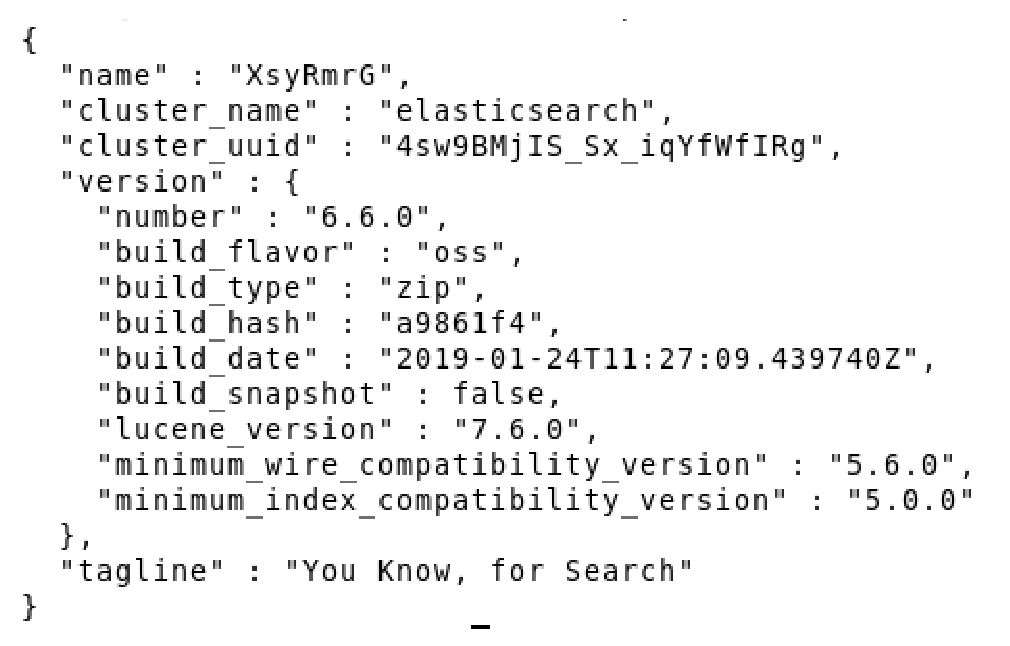
\includegraphics[width=\textwidth, height=\textheight]{imagens/pretty.eps}
		%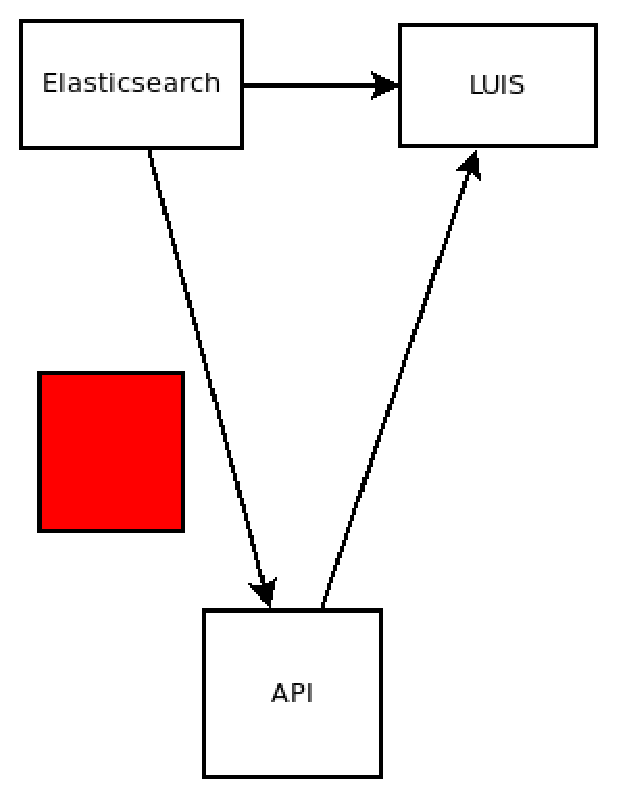
\includegraphics[width=0.5\textwidth, height=0.35\textheight]{imagens/teste.eps}
                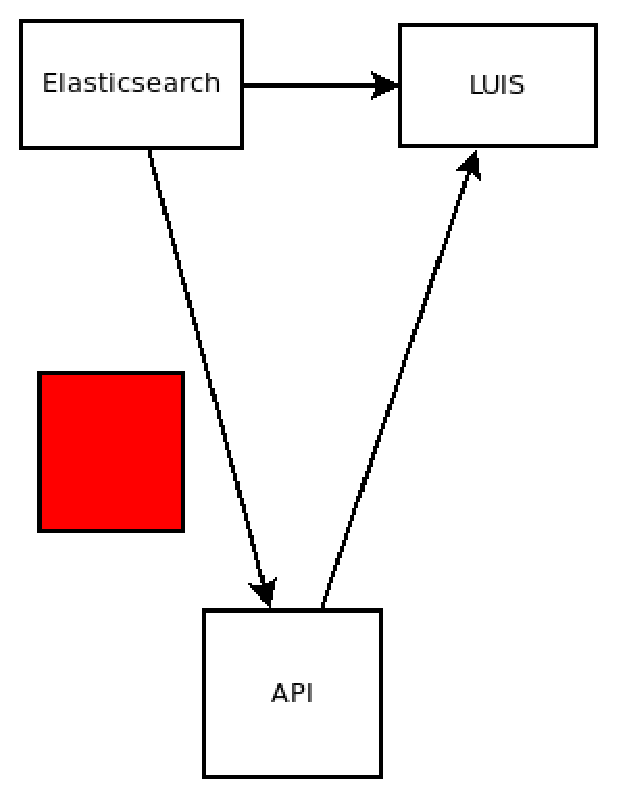
\includegraphics[width=\textwidth]{imagens/teste.eps}
        \end{center}
        \legend{Fonte: Autor}
\end{figure}


% ---

% ---
%\section{Aliquam vestibulum fringilla lorem}
% ---

% ----------------------------------------------------------
% PARTE
% ----------------------------------------------------------
%\part{Resultados}
% ----------------------------------------------------------

% ---
% primeiro capitulo de Resultados
% ---
%\chapter{Lectus lobortis condimentum}
% ---

% ---
%\section{Vestibulum ante ipsum primis in faucibus orci luctus et ultrices posuere cubilia Curae}
% ---

% ---
% segundo capitulo de Resultados
% ---
%\chapter{Nam sed tellus sit amet lectus urna ullamcorper tristique interdum elementum}
% ---

% ---
%\section{Pellentesque sit amet pede ac sem eleifend consectetuer}
% ---

% ----------------------------------------------------------
% Finaliza a parte no bookmark do PDF
% para que se inicie o bookmark na raiz
% e adiciona espaço de parte no Sumário
% ----------------------------------------------------------
\phantompart

% ---
% Conclusão
% ---
%\chapter{Conclusão}
% ---

% ----------------------------------------------------------
% ELEMENTOS PÓS-TEXTUAIS
% ----------------------------------------------------------
\postextual
% ----------------------------------------------------------

% ----------------------------------------------------------
% Referências bibliográficas
% ----------------------------------------------------------
\bibliography{elementos/bibliografia.bib}

% ----------------------------------------------------------
% Glossário
% ----------------------------------------------------------
%
% Consulte o manual da classe abntex2 para orientações sobre o glossário.
%
%\glossary

% ----------------------------------------------------------
% Apêndices
% ----------------------------------------------------------

% ---
% Inicia os apêndices
% ---
%\begin{apendicesenv}

% Imprime uma página indicando o início dos apêndices
%\partapendices

% ----------------------------------------------------------
%\chapter{Quisque libero justo}
% ----------------------------------------------------------

% ----------------------------------------------------------
%\chapter{Nullam elementum urna vel imperdiet sodales elit ipsum pharetra ligula ac pretium ante justo a nulla curabitur tristique arcu eu metus}
% ----------------------------------------------------------
%\end{apendicesenv}
% ----------------------------------------------------------


% ----------------------------------------------------------
% Anexos
% ----------------------------------------------------------

% ---
% Inicia os anexos
% ---
%\begin{anexosenv}

% Imprime uma página indicando o início dos anexos
%\partanexos

% ---
%\chapter{Morbi ultrices rutrum lorem.}
% ---

% ---
%\chapter{Cras non urna sed feugiat cum sociis natoque penatibus et magnis dis parturient montes nascetur ridiculus mus}
% ---

% ---
%\chapter{Fusce facilisis lacinia dui}
% ---
%\end{anexosenv}

%---------------------------------------------------------------------
% INDICE REMISSIVO
%---------------------------------------------------------------------
\phantompart
\printindex
%---------------------------------------------------------------------

\end{document}
